\documentclass{beamer}
\usepackage[spanish]{babel}
\usepackage[utf8]{inputenc}
\usepackage{units}
\usetheme{Antibes}
\usepackage{tikz}
\usecolortheme{albatross}
\usefonttheme{professionalfonts}
\AtBeginDocument{%
  \renewcommand\figurename{Referencia}
}
\usepackage{caption}
\usepackage{subcaption}
\setbeamertemplate{navigation symbols}{}


\title[MIFSA: Herramienta para análisis de espectros]{MIFSA: Herramienta para análisis de espectros}
\subtitle{Análisis de cubos de datos de CALIFA}
\author[Julián Jiménez-Cárdenas, Sebastián Ordóñez-Soto]{Julián Jiménez Cárdenas$^{1}$, Sebastián Ordóñez-Soto$^1$}
\institute{$^{1}$Estudiante de Física, Universidad Nacional de Colombia \and \texttt{juojimenezca@unal.edu.co\\ jsordonezs@unal.edu.co}\and \texttt{https://github.com/julian20250/MIFSA}}
\date{17 de Septiembre del 2016}
\begin{document}
	\frame{\titlepage}
	\begin{frame}
		\frametitle{Índice}
		\tableofcontents		
	\end{frame}
	\section{Espectro Electromagnético}
	\subsection{Introducción}
	\begin{frame}
	\frametitle{Introducción}
	\begin{figure}
	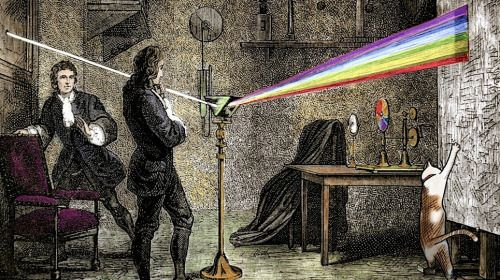
\includegraphics[width=.8\textwidth]{newton}
	\caption{\tiny{\url{https://s-media-cache-ak0.pinimg.com/564x/30/66/42/306642ae81b1a73f0f9a6d4937b4472a.jpg}}}
	\end{figure}
	\end{frame}
	\begin{frame}
	\frametitle{Ondas}
	\begin{figure}
\centering
\begin{subfigure}{.5\textwidth}
  \centering
  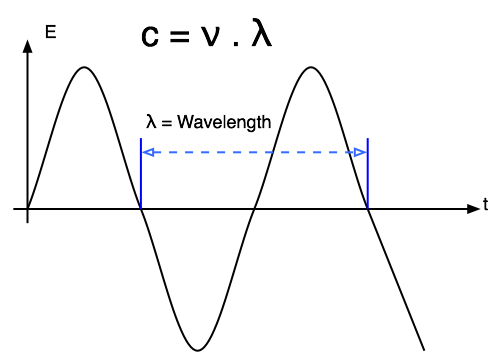
\includegraphics[width=1\linewidth]{wavelength}
  \caption{\tiny{\url{https://upload.wikimedia.org/wikipedia/commons/4/4a/Espejo_(3207185886).jpg}}}
  \label{fig:sub1}
\end{subfigure}%
\begin{subfigure}{.5\textwidth}
  \centering
  \includegraphics[width=1\linewidth]{mechanic}
  \caption{\tiny{\url{http://escience.anu.edu.au/lecture/cg/Color/Image/waveLength.png}}}
  \label{fig:sub2}
\end{subfigure}

\label{fig:test}
\end{figure}
	\end{frame}
	
	%?=============
		\subsection{¿Qué es el espectro?}
	\begin{frame}
	\frametitle{¿Qué es el espectro?}
	\begin{figure}
	

	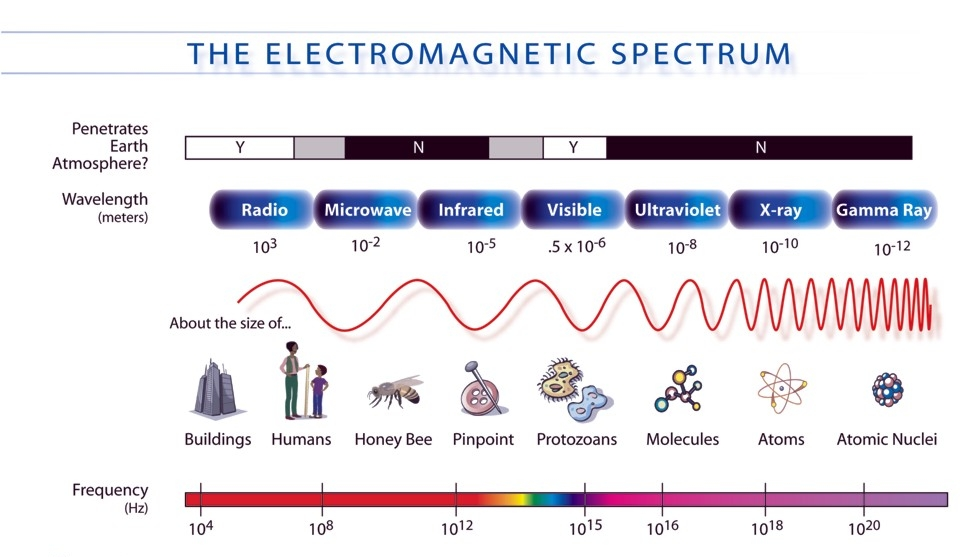
\includegraphics[width=\textwidth]{longitudes}
	
	\caption{\tiny{\url{http://www.photobiology.org/UserFiles/Image/EM-spectrum.jpg}}}
	\end{figure}

	\end{frame}

	\begin{frame}
	\frametitle{Espectros de estrellas}
	\begin{figure}
	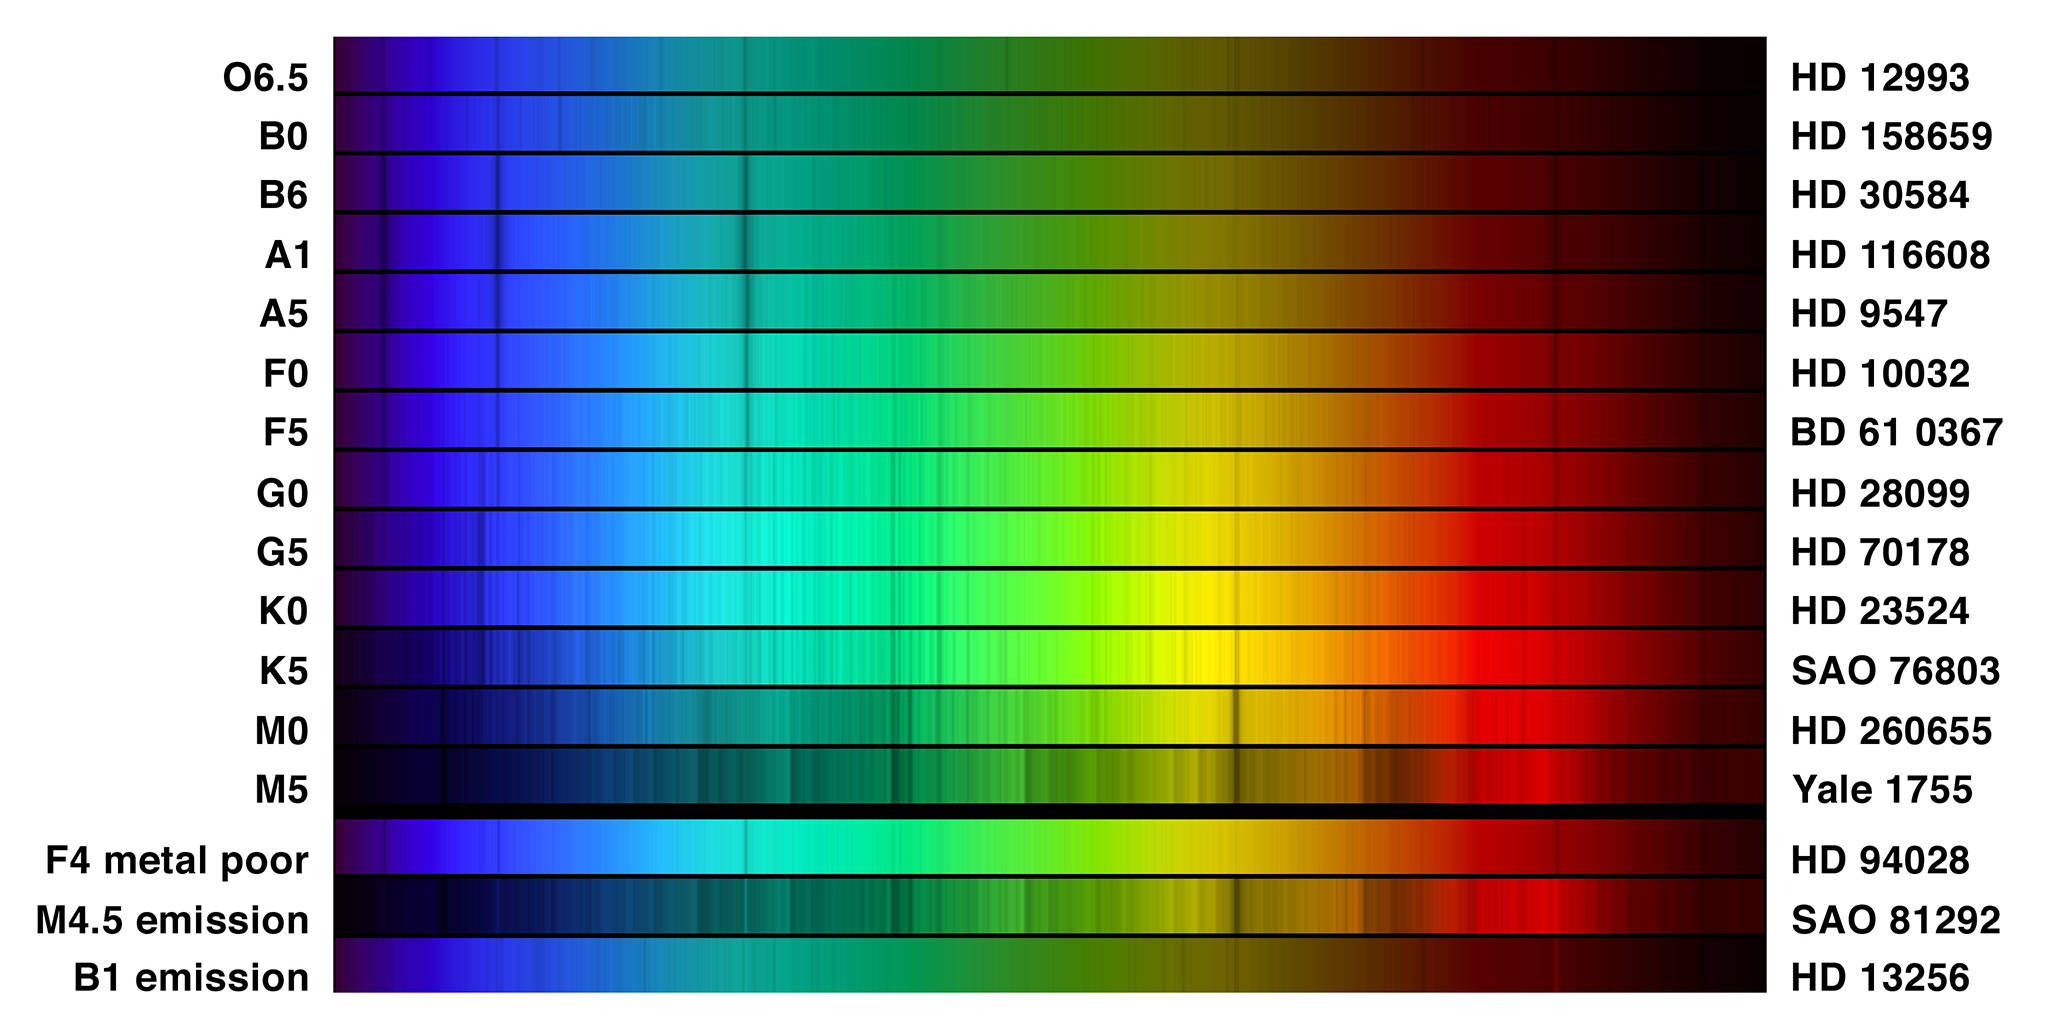
\includegraphics[width=\textwidth]{StellarSpectrum}
	\caption{\tiny{\url{http://www.extrasolar.de/wp-content/uploads/2016/05/Spectrum.jpg}}}
	\end{figure}

	\end{frame}
	\begin{frame}
	\frametitle{Emisión y Absorción}
	\begin{figure}
	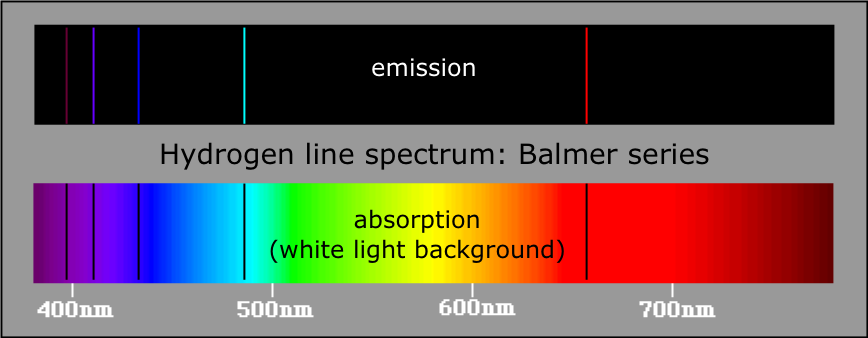
\includegraphics[width=\textwidth]{emision-absorcion}
	\caption{\tiny{\url{http://casanchi.com/did/espectro04.jpg}}}
	\end{figure}
	\end{frame}
	\begin{frame}
	\frametitle{Espectro NGC2410}
	\begin{figure}
	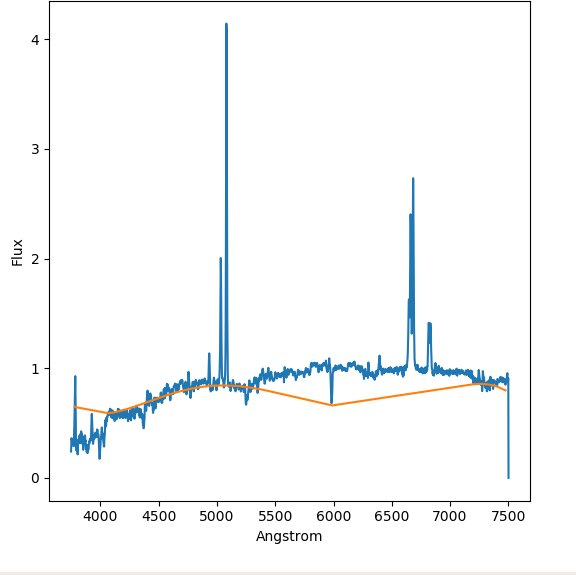
\includegraphics[width=.5\textwidth]{output}
	\end{figure}
	\end{frame}
	\section{Python}
	\begin{frame}
	\frametitle{Python}
	\begin{figure}
	
\includegraphics[width=\textwidth]{python}
	\caption{\tiny{\url{https://cdn.fedoramagazine.org/wp-content/uploads/2015/11/Python_logo.png}}}
	\end{figure}
	\end{frame}
	\subsection{Numpy}
	\begin{frame}
	\frametitle{Numpy}
	\begin{figure}
	
\includegraphics[width=.5\textwidth]{numpy}
	\caption{\tiny{\url{https://bids.berkeley.edu/sites/default/files/styles/400x225/public/projects/numpy_project_page.jpg?itok=flrdydei}}}
	\end{figure}
	
	\end{frame}			
	\subsection{Matplotlib}
	\begin{frame}
	\frametitle{Matplotlib}
	\begin{figure}
	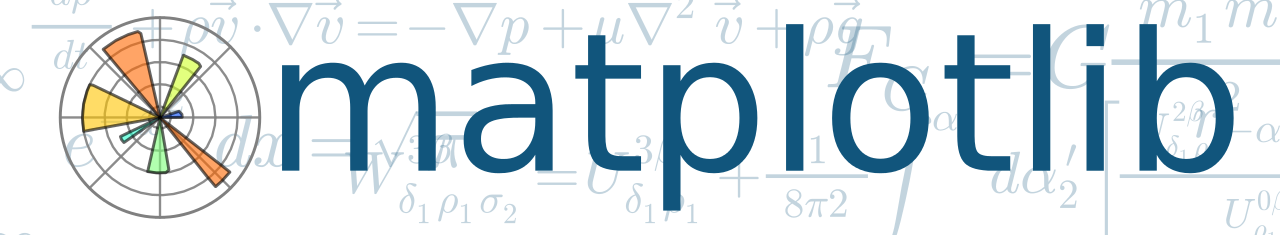
\includegraphics[width=\textwidth]{matplotlib}
	\caption{\tiny{\url{https://upload.wikimedia.org/wikipedia/en/thumb/5/56/Matplotlib_logo.svg/1280px-Matplotlib_logo.svg.png}}}
	\end{figure}
	\end{frame}
	\section{MIFSA}
	\subsection{Califa}
	\begin{frame}
	\frametitle{Calar Alto Legacy Integral Field spectroscopy Area survey}
	\begin{figure}
	\includegraphics[height=.75\textheight]{califa}
	\caption{\tiny{\url{https://upload.wikimedia.org/wikipedia/commons/6/6e/CALIFA_HexDR2_mandala.png}}}
	\end{figure}
	\end{frame}
	\begin{frame}
	\frametitle{Map
Integral Field Spectroscopy Analysis}
\begin{figure}
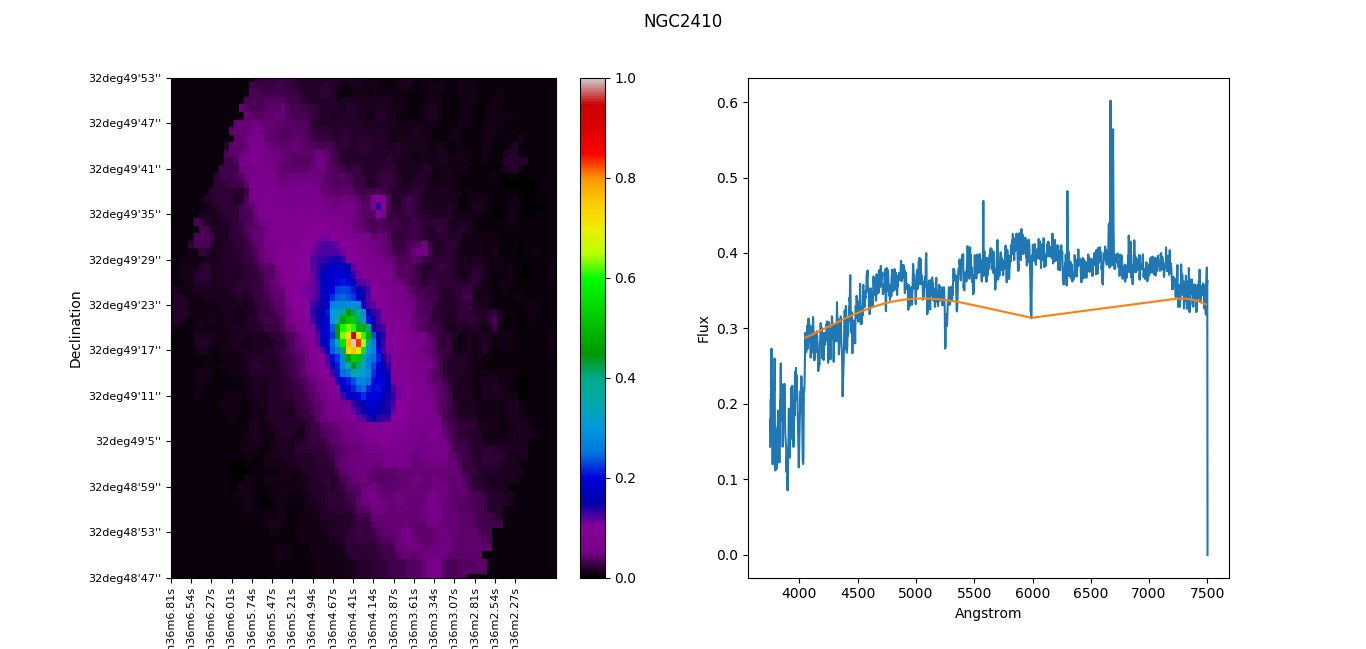
\includegraphics[width=\textwidth]{fullOutput}
\end{figure}
	\end{frame}
\end{document}